\documentclass[a4paper,12pt]{article} % тип документа
\usepackage[margin=1in]{geometry} % Поля

%  Русский язык
\usepackage[warn]{mathtext}
\usepackage[T2A]{fontenc}			% кодировка
\usepackage[utf8]{inputenc}			% кодировка исходного текста
\usepackage[english,russian]{babel}	% локализация и переносы
% Математика
\usepackage{amsmath,amsfonts,amssymb,amsthm,mathtools} 
\usepackage{wasysym}
%%%
\usepackage{graphicx}

\usepackage{tabularx}

\usepackage{gensymb} % знак градуса
\usepackage{enumitem} % изменить список enumerate
\usepackage{placeins} % \FloatBarrier

\renewcommand{\thesection}{\Roman{section}} 
\renewcommand{\thesubsection}{\roman{subsection}}


\begin{document}

\newcolumntype{Y}{>{\centering\arraybackslash}X} %new tabularx


%титул
\hrule 	
\medskip
\begin{raggedright}
{\large \textbf{Вопрос по выбору}}
\\
\medskip
{\Large Симметрии в стандартной модели} 
\\
\medskip
{\large Карташов Констанин Б04-005}
\medskip
\hrule
\medskip
\end{raggedright}


\section{Обзор стандартной модели}

\paragraph{} Физика элементарных частиц на сегодняшний день прекрасно описывается стандартной моделью (СМ) фундаментальный взаимодействий, которая аккумулирует в себе все достижения последних лет. Под стандартной моделью подразумевается квантово-полевая теория, которая описывает микромир на самом фундаментальном известном на сегодня уровне. При этом элементарными полями в СМ являются кварки и лептоны, которые участвуют в четырёх видах взаимодействий: сильном, слабом, электромагнитном и юкавском, осуществляемых обменом квантами соответствующих полей. В СМ присутствует также поле спина нуль, называемое хиггсовским бозоном, взаимодействие с которым обеспечивает массы всех элементарных частиц. Гравитация, не входит в СМ.

\paragraph{} К фермионам относятся кварки трёх поколений: \textbf{u} и \textbf{d} -- первое, \textbf{c} и \textbf{s} -- второе, \textbf{t} и \textbf{b} -- третье, кварки типа \textbf{u} имеют проекцию слабого изоспина (слабого изотопического спина) $I_3 = +1/2$ и электрический заряд $Q = +2/3$, для кварков типа \textbf{d}: $I_3 = -1/2$, $Q = -1/3$. Кварк также имеет один из трёх цветовых зарядов (\textit{к, с, з}), и соответствующий ему анти-кварк.

Также к фермионам относится три поколения лептона: \textbf{электрон} и \textbf{электронное нейтрино}, \textbf{мюон} и \textbf{мюонное нейтрино}, \textbf{тау-лептон} и \textbf{тау-нейтрино}. Лептоны типа электрона имеют электрически заряд $Q = -1$ и проекцию слабого изоспина $I_3 = +1/2$, нейтрино имеют $Q = 0$ и $I_3 = -1/2$.

\paragraph{} К калибровочным бозонам относятся: фотоны -- переносчики электромагнитного взаимодействия, $Z^0, W^{\pm 1}$ бозоны -- переносчики слабого взаимодействия, глюоны 8 типов -- переносчики сильного взаимодействия. Также в СМ входит скалярный бозон Хиггса -- определяющий массы элементарных частиц.

\begin{figure}[h]
\centering
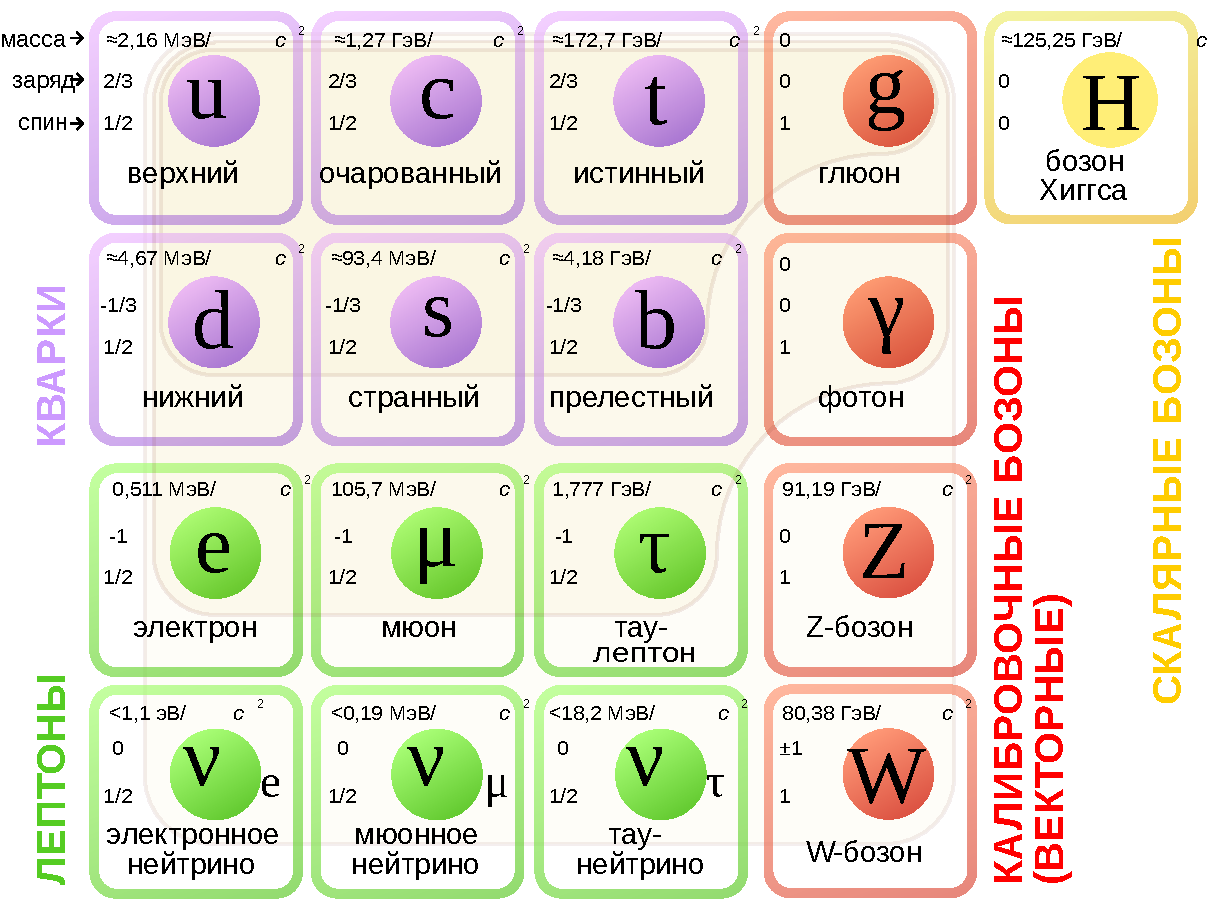
\includegraphics[width=0.6\textwidth]{sm_chart_ru.pdf}
\caption{Элементарные частицы стандартной модели}
\label{fig:sm_chart}
\end{figure}

\medskip\hrule\medskip

\section{Симметрии стандартной модели}

\paragraph{} Многие предсказания СМ строятся на сохранении определённых симметрий. Симметриями в квантовой теории поля называются преобразования координат и (или) полевых функций, относительно которых инвариантны уравнения движения, а значит, инвариантно действие. Сами преобразования при этом образуют группу. Симметрии называются глобальными, если соответствующие преобразования не зависят от 4-координат. В противном случае говорят о локальных симметриях. Группы преобразований обычно рассматриваются в некотором представлении — элементам групп соответствуют операторные (матричные) функции параметров. 

\subsection{\textit{CPT}-теорема}

\paragraph{} Рассмотрим симметрии природы, связанные с возможностью замены правого на левое, частицы на античастицу и обращения времени. Оказывается, что все три операции -- зарядового сопряжения $\hat{C}$ (замены частиц античастицами), пространственной инверсии $\hat{P}$ (замены координаты $\mathbf{r}$ на $-\mathbf{r}$) и обращения времени $\hat{T}$ (замены времени $t$ на $-t$), взятые вместе не являются совсем независимыми. Произведённые последовательно друг на другом, преобразования $\hat{C}$, $\hat{P}$, $\hat{T}$ обязаны не менять никаких следствия теории (т.е. $\hat{C} \hat{P} \hat{T} = 1$ ). Это утверждение носит название \textit{CPT}-теоремы.

Из \textit{CPT}-теоремы, в частности следует, что массы и времена жизни частицы и античастицы равны, магнитные моменты различаются только знаком, взаимодействие частицы и античастицы с гравитационным полем одинаково. На опыте не обнаружено ни одного случая нарушения \textit{CPT}-инвариантности.

В то же время мы теперь знаем, что в слабых взаимодействиях нарушаются как \textit{P}-  и \textit{C}-инвариантности, так и \textit{CP-}инвариантность. Несохранение чётности было обнаружено в 1957 г. в $\beta$-распаде $^{60}$Co.

\subsection{Локальная калибровочная U(1)-симметрия} \label{ss:u1}

\paragraph{} Унитарная группа первого порядка U(1) в математике -- группа преобразований полученных умножением на комплексное число по модулю равном единице: $ e^{i \alpha} $. В контексте теории поля такое преобразование имеет смысл смещения фазы волновой функции, в при сохранении локальной симметрии это преобразование может зависеть от 4-координаты: $e^{i \alpha(x^\mu)}$. 

В качестве примера рассмотрим комплексное скалярное поле $\phi(x^\mu)$. Лагранжиан (плотность лагранжиана) скалярного поля: 

\begin{equation}
\mathcal{L}_\text{scalar}(\phi) = \partial_\mu \phi^* \partial^\mu \phi - m^2 \phi^* \phi.
\label{e:scal_field}
\end{equation}

При применении преобразование $\phi' = e^{iq\alpha(x^\mu)} \phi, \phi'^* = e^{-iq\alpha(x^\mu)} \phi$, в лагранжиане возникают члены $\partial_m \alpha(x^\mu)$. Для сохранения ковариантности можно ввести свободное калибровочное поле $A^\mu$, и переписать лагранжиан \eqref{e:scal_field} при помощи калибровочно-ковариантной производной:

\begin{equation}
D_\mu = \partial_\mu - iqA^\mu.
\label{e:diff_cov}
\end{equation}

Согласно общему подходу для свободного калибровочного поля $A^\mu$ также необходимо ввести калибровочно-инвариантный лагранжиан, который согласно общему подходу равен:

\begin{equation}
\mathcal{L}_f = - \frac{1}{4} F^{\mu \nu}F_{\mu \nu}, \; F_{\mu \nu} = \partial_\mu A_\nu - \partial_\nu A_\mu.
\label{e:f_lagr}
\end{equation}

Учитывая \eqref{e:scal_field}, \eqref{e:diff_cov} и \eqref{e:f_lagr} получим лагранжиан для скалярного поля с локальной калибровочной U(1)-симметрией:

\begin{equation}
\mathcal{L} = (D_\mu \phi)^* D^\mu \phi - m^2 \phi^* \phi - \frac{1}{4} F^{\mu \nu}F_{\mu \nu}.
\label{e:cov_lagr}
\end{equation}

Таким образом требование локальной калибровочной U(1)-симметрии приводит к появлению калибровочного поля, например электромагнитного, и соответствующему ему калибровочному бозону - фотону. Локальная U(1)-симметрия также влечёт за собой глобальную U(1)-симметрию, что по тереме Нётер приводит к закону сохранения заряда (электрического, барионного, странности и т.д.)

\subsection{Локальная калибровочная SU(3)-симметрия} \label{ss:su3}

\paragraph{} Специальная унитарная группа порядка n SU(n) -- группа преобразований осуществляемых унитарной матрицей $n\times n$ с определителем равным 1. Наблюдение SU(3)-симметрии в элементарных частицах стало основанием для предсказания предсказания новых элементарных частиц, создание кварковой модели, и создание в итоге квантовой хромодинамики. 

\begin{figure}[h]
\centering
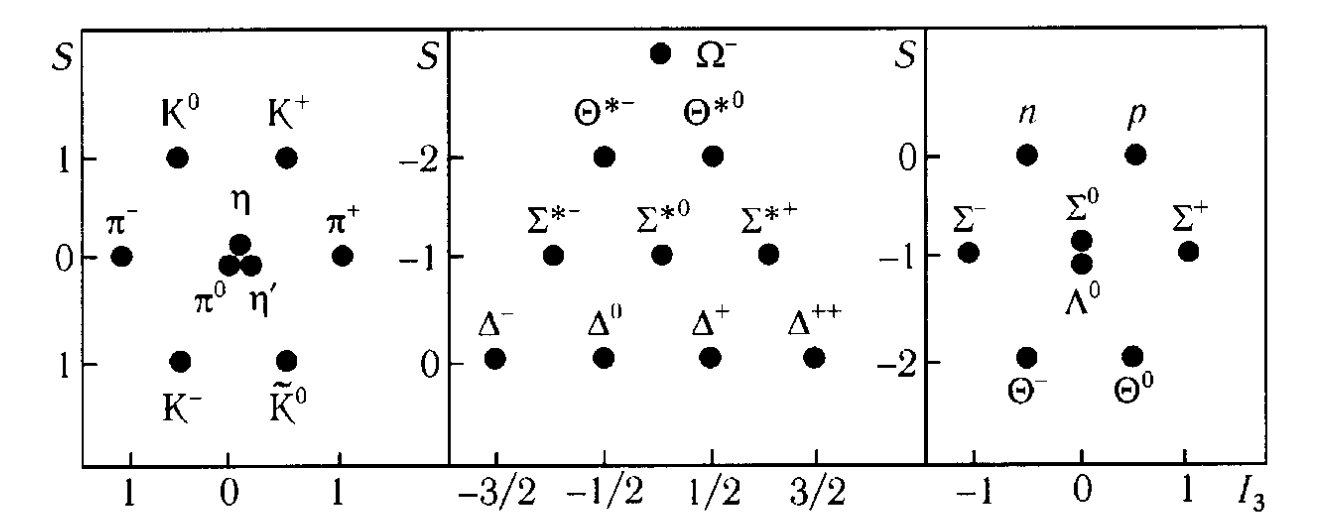
\includegraphics[width=\textwidth]{unitary_singlets.png}
\caption{Унитарные синглеты адронов: нонет мезонов, октет барионов, декуплет барионов}
\label{fig:unitary_singlets}
\end{figure}

\paragraph{} Внимательное рассмотрение обычных и странных адронов позволило выяснит, что изотопические мультиплеты, в свою очередь группируются в ещё большие семейства - унитарные мультиплеты. На плоскости ($S$, $I_3$) (странность, проекция изоспина) эти группы располагаются в виде симметричных относительно поворота на $120\degree$ фигур (рис. \ref{fig:unitary_singlets}). В 1961 г. М. Гелл-Маном и Ю. Нееманом была предложена SU(3)-симметрия. Одним из простейших представлением SU(3) группы является триплет в состав которого входит частица со странностью, отличной от нуля. Мезонные нонеты в SU(3)-симметрии получаются как комбинация триплета с <<антитриплетом>>, а барионные декуплеты -- при комбинировании трёх триплетов.

На основании этой модели в 1964 г. М. Гелл-Ман и Г.Цвейг независимо сделали предположение о существовании в природе частиц с дробными значениями барионного числа и электрического заряда -- названые в итоге кварками.

\paragraph{} Квантовая хромодинамика — неабелева калибровочная теория с SU(3) группой симметрии. Она описывает дираковкие поля $\psi^i, i=1,2,3$, которые представляют кварковые поля и векторные поля $A^{a \mu}, a=1,...,8$ -- глюонные поля, которые являются SU(3) калибровочными бозонами.

\paragraph{} В стандартной модели SU(3)-симметрия проявляет себя как закон сохранения цветового заряда, и экранирование кварков и глюонов внутри адронов (невозможность наблюдения <<цветных>> частиц) 

\subsection{Локальная калибровочная SU(2)-симметрия} \label{ss:su2}

\paragraph{} SU(2)-симметрия подобна SU(3)-симметрии. SU(2)-симметрия проявляет себя через наличие кварк-лептонных дублетов:

\[
\left( \begin{array}{c} \nu_e \\ e^- \end{array} \right) \rightarrow \left( \begin{array}{c} u \\ d \end{array} \right); \;\;\;
\left( \begin{array}{c} \nu_\mu \\ \mu^- \end{array} \right) \rightarrow \left( \begin{array}{c} c \\ s \end{array} \right); \;\;\;
\left( \begin{array}{c} \nu_\tau \\ \tau^- \end{array} \right) \rightarrow \left( \begin{array}{c} t \\ b \end{array} \right), \;\;\;
\]

\noindent что истолковывается как отражение существования особого квантового числа -- слабого изоспина $I_3 = 1/2$. Каждый дублет соответствует поколению фермионов.

\paragraph{} В стандартной модели калибровочное поле соответствующее SU(2)-симметрии -- поле слабого взаимодействия ($W^\pm$, $Z^0$ бозоны). При этом в СМ SU(2)-симметрия применима только к левосторонним фермионам (или правосторонним анти-фермионам), существование правосторонних фермионов экспериментально не доказано, однако открытие нейтринных осцилляций, не описываемых СМ, может означать их существование. 

\medskip\hrule\medskip

\end{document}
